\documentclass[tikz]{standalone}
\usetikzlibrary{calc,arrows}
\usepackage{amsmath}
\usepackage{mathabx}

\begin{document}
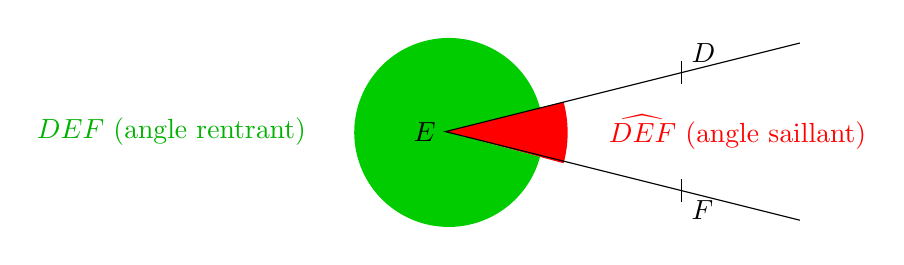
\begin{tikzpicture}[scale=1.5]
    \coordinate (E) at (0,0);
    \coordinate (D) at (2,0.5);
    \coordinate (F) at (2,-0.5);
    \fill[red] (E) -- ($(E)!0.5!(D)$) arc(15:-15:1) -- cycle;
    \fill[green!80!black] (E) -- ($(E)!0.4!(D)$) arc(15:345:0.8) -- cycle;
    \draw ($(E)!1.5!(D)$) -- (E) -- ($(E)!1.5!(F)$);
    \draw ($(D)+(0,0.1)$) -- ($(D)+(0,-0.1)$);
    \draw ($(F)+(0,0.1)$) -- ($(F)+(0,-0.1)$);
    \node[above right] at (D) {$D$};
    \node[below right] at (F) {$F$};
    \node[left] at (E) {$E$};
    \node[red, anchor=west] at (1.3,0) {$\widehat{DEF}$ (angle saillant)};
    \node[green!70!black, anchor=east] at (-1.1,0) {$\widecheck{DEF}$ (angle rentrant)};
\end{tikzpicture}
\end{document}